\documentclass[main]{IEEEtran}
\IEEEoverridecommandlockouts
% The preceding line is only needed to identify funding in the first footnote. If that is unneeded, please comment it out.
\usepackage{cite}
\usepackage{amsmath,amssymb,amsfonts}
\usepackage{algorithmic}
\usepackage{graphicx}
\usepackage{textcomp}
\usepackage{xcolor}
\usepackage[UTF8]{ctex}  % 支持中文
\usepackage{titlesec}    % 加载titlesec宏包,自定义标题样式
\usepackage{float}
\usepackage{booktabs}
\usepackage{siunitx}   % 使用 siunitx 包来帮助对数字进行对齐
\usepackage{hyperref}


\renewcommand{\figurename}{图}            % 控制图片标题前缀,如“图 1”
\renewcommand{\figureautorefname}{图}     % 控制 \autoref{fig:xxx} 的引用前缀

\renewcommand{\tablename}{表}
\renewcommand{\tableautorefname}{表}



\hypersetup{
    colorlinks=true,      % 设置超链接为彩色
    linkcolor=blue,       % 内部链接颜色,例如\ref命令生成的链接
    citecolor=green,      % 引用链接颜色,如文献引用
    filecolor=magenta,    % 文件链接颜色
    urlcolor=cyan,        % 外部URL链接颜色
}

\renewcommand{\refname}{参考文献}

% 重定义摘要名称和摘要内容的格式
\renewcommand{\abstractname}{\zihao{5}\heiti 摘要}  % 摘要标题为5号黑体
% 重定义关键词标题
\renewcommand{\IEEEkeywordsname}{关键词}
% 重定义关键词名称和内容的格式
\renewcommand{\IEEEkeywordsname}{\zihao{5}\heiti 关键词}  % 关键词标题为5号黑体
% 设置标题为4号宋体
\title{\zihao{4}\songti 标题(一级标题,4号宋体)}

\usepackage[labelsep=period]{caption}
\DeclareCaptionLabelFormat{myformat}{#1 #2}
\captionsetup[figure]{labelformat=myformat}

%\usepackage[labelsep=period]{caption}
\DeclareCaptionLabelFormat{myformat}{#1 #2}
\captionsetup[table]{labelformat=myformat}

% 设置节标题样式为阿拉伯数字,并使其靠左对齐
\titleformat{\section}
{\normalfont\Large\bfseries}{\thesection.}{0.5em}{}
\renewcommand{\thesection}{\arabic{section}} % 使用阿拉伯数字编号

% 设置二级节标题样式为5号黑体,并使其靠左对齐,格式为“1.1 标题”
\titleformat{\subsection}
{\normalfont\large\bfseries}{\thesubsection}{0.5em}{}
\renewcommand{\thesubsection}{\thesection.\arabic{subsection}} % 使用“1.1”等格式

% 设置三级节标题样式为5号宋体,并使其靠左对齐
\titleformat{\subsubsection}
{\normalfont\zihao{5}\songti\flushleft}{\thesubsubsection}{1em}{}

% 重新定义三级节的编号格式为“1.1.1”
\renewcommand{\thesubsubsection}{\thesubsection.\arabic{subsubsection}}

% 设置一级节标题样式为4号宋体,并使其靠左对齐
\titleformat{\section}
{\normalfont\zihao{4}\songti\bfseries}{\thesection.}{0.5em}{}

% 设置二级节标题样式为5号黑体,并使其靠左对齐
\titleformat{\subsection}
{\normalfont\zihao{5}\heiti\bfseries}{\thesubsection}{0.5em}{}


\def\BibTeX{{\rm B\kern-.05em{\sc i\kern-.025em b}\kern-.08em
T\kern-.1667em\lower.7ex\hbox{E}\kern-.125emX}}
\begin{document}
\pagestyle{plain}  % 使用 plain 样式,页码位于页脚居中


\title{
对抗性学习攻击

{\footnotesize \textsuperscript{} 万杰 3124357005 17364521744 选修课}
}
\maketitle
\thispagestyle{plain}
\pagestyle{plain}
\begin{abstract}
    \zihao{5}\kaishu  % 摘要使用5号楷体
本文系统阐述了对抗样本攻击在视觉、语音和文本三个领域的技术细节与典型案例,并从攻击原理、攻击危害和防御措施三个层面展开全面分析。在视觉领域,像素级扰动和对抗补丁等方法能够使自动驾驶系统错误识别交通标志,威胁行车安全;在语音领域,高频扰动与隐蔽语音命令可能让语音助手在用户不知情的情况下执行恶意操作;在文本领域,通过细微的同义词替换或字符修改即可造成情感分析与审核系统的严重误判。随后,文章详细介绍了针对三大领域的常见防御策略,包括对抗训练、输入预处理以及可证鲁棒性等方法,并在最后结合应用场景的需求与实际落地困难,对该技术的未来发展提出个人见解。
\end{abstract}

\begin{IEEEkeywords}
    \zihao{5}\kaishu  % 摘要使用5号楷体
 对抗样本攻击,深度学习安全,视觉攻击,语音攻击,文本攻击
\end{IEEEkeywords}


\section{技术细节}
\subsection{攻击原理}
对抗样本攻击旨在利用模型在高维输入空间的脆弱性,通过对原始输入添加微小扰动,使得模型的决策边界发生显著偏移。虽这些扰动对人类几乎不可见或难以察觉,但对于深度模型的神经元激活却具有严重的扰动效果,足以使模型在推理时输出严重的错误结果\cite{goodfellow2014explaining}。

\subsection{视觉领域对抗攻击}
视觉领域是对抗样本研究最早且最成熟的应用场景之一,主要集中在图像分类、目标检测、图像分割等任务中。

像素级扰动:在ImageNet数据集上,加入小到不可见的像素噪声即可使CNN模型产生错误分类\cite{goodfellow2014explaining}。该攻击方式的核心难点是 如何将扰动控制在极小范围内,同时保证较高的成功率。

对抗补丁(Adversarial Patch):在图像的一小块区域(Patch)上添加可见扰动\cite{brown2017adversarial}。 此类攻击在自动驾驶和安防系统中尤具威胁,攻击者无需全局修改图像,只需在部分区域添加扰动即可。

物理世界攻击:现实世界中,交通标志上贴纸或者喷涂特殊图案,导致自动驾驶系统错误识别交通信号,从而导致交通事故\cite{kurakin2018adversarial}。

\subsection{语音领域对抗攻击}
语音指令攻击: 通过对音频信号植入细微扰动,实现“隐藏语音命令”(Hidden Voice Commands),让语音助手在用户不知情的情况下执行恶意操作\cite{carlini2018audio}。该攻击方式 通常利用频域或时域上对原始音频的梯度信息进行微调,使听觉上无明显失真,但语音识别系统却会将其解码为任意文本指令。

超声波攻击: 该攻击方式通常将指令信号嵌入到超声波或高频范围中,利用麦克风的非线性失真特性在可听范围内还原攻击内容\cite{song2017poster}。因为人耳正常无法 听到此类高频声波,因此该攻击方式隐蔽性极高。

\subsection{文本领域对抗攻击}
自然语言处理(NLP)在文本分类、情感分析、机器翻译等任务上取得突破,但也面临文本对抗攻击的威胁。

字符级扰动:例如HotFlip攻击通过对文本中的字符进行最小替换来诱导模型产生错误预测\cite{ebrahimi2017hotflip}。该攻击方式的难点在于需要保证文本在语义和可读性上保持一致,不能被轻易察觉。

同义词替换和语义级攻击:该攻击方式通常通过 在句子中替换同义词或同义短语,在保证可读性和语义一致的情况下实现攻击。例如TextBugger、DeepWordBug等通过对词和短语进行扰动,攻击文本分类和情感分析模型\cite{li2019textbugger}。

\section{攻击案例}

\subsection{视觉领域攻击案例}
\subsubsection{图像分类错误案例}

在经典的ImageNet数据集上,研究人员通过添加微小扰动实现了使深度卷积神经网络(CNN)错误分类的攻击。常见的对抗样本如“熊猫”被判定为“长臂猿”,甚至只需改变少量像素即可迷惑模型\cite{goodfellow2014explaining}。

\begin{figure}[H]
    \centering
    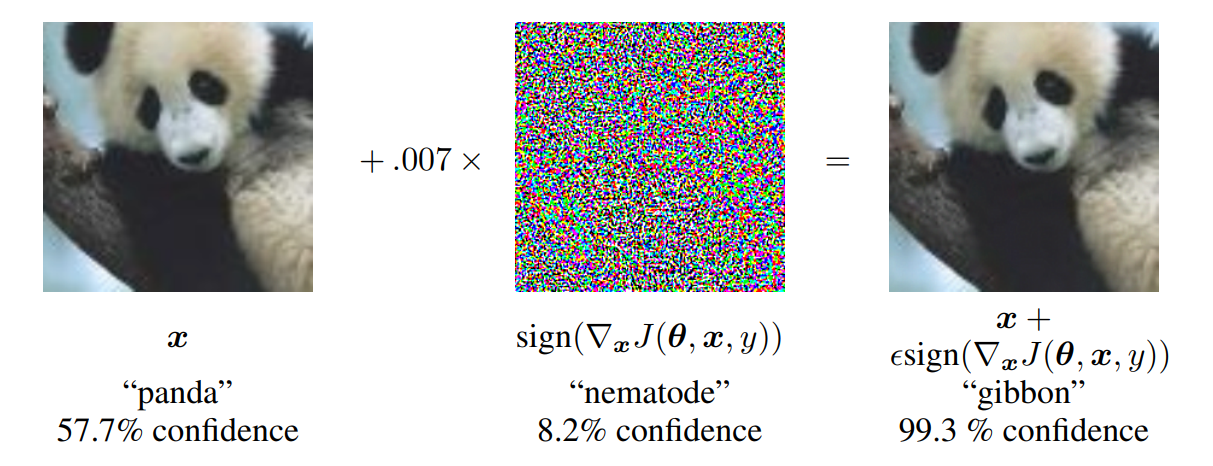
\includegraphics[height=3.5cm]{fig/p_to_g}
    \caption{“熊猫”被判定为“长臂猿”}
    \label{fig:p_to_g}
\end{figure}

如\autoref{fig:p_to_g}所示,左图为原始“熊猫”图像;中间经过微小扰动处理;右图虽然肉眼几乎看不出明显变化,但深度学习模型输出已从“Panda”错误地变为“Gibbon”。

\subsubsection{对抗补丁案例}
对抗补丁(Adversarial Patch)只需在图像某一小块区域添加可见扰动贴纸,便可在物理世界中有效迷惑识别系统\cite{brown2017adversarial},这在自动驾驶场景中尤具威胁。

\begin{figure}[H]
    \centering
    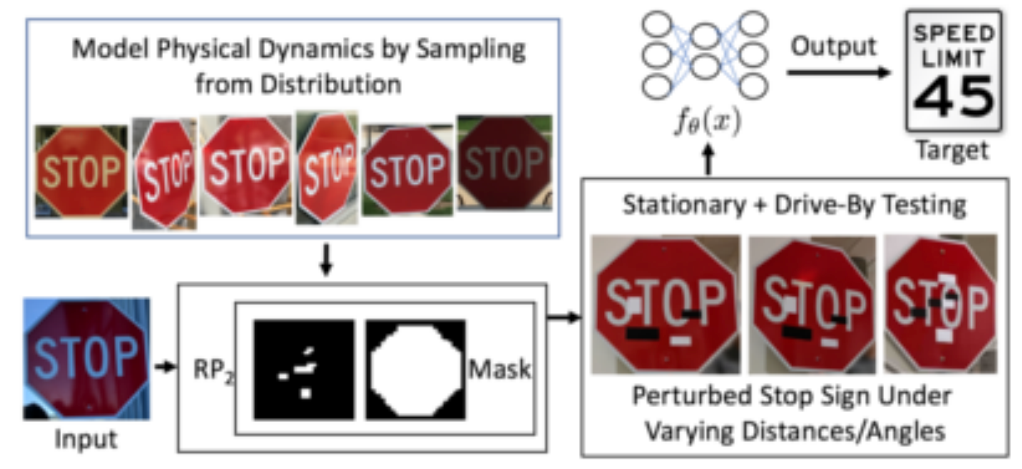
\includegraphics[height=3.5cm]{fig/stop}
    \caption{停车标志识别成限速标志}
    \label{fig:stop}
\end{figure}

如\autoref{fig:stop}所示,在停车标志上贴一个小贴纸便可能使摄像头误识别为限速标志\cite{eykholt2018robust}。



\subsection{语音领域攻击案例}
\subsubsection{隐蔽语音命令}
通过在音频信号中加入针对语音识别系统的扰动,使人耳几乎无法察觉,但系统却解码为恶意指令\cite{carlini2018audio}。如\autoref{fig:yuying}所示,只是在原有的音频信号上添加了微小扰动,语音系统就无法正确识别。

\begin{figure}[H]
    \centering
    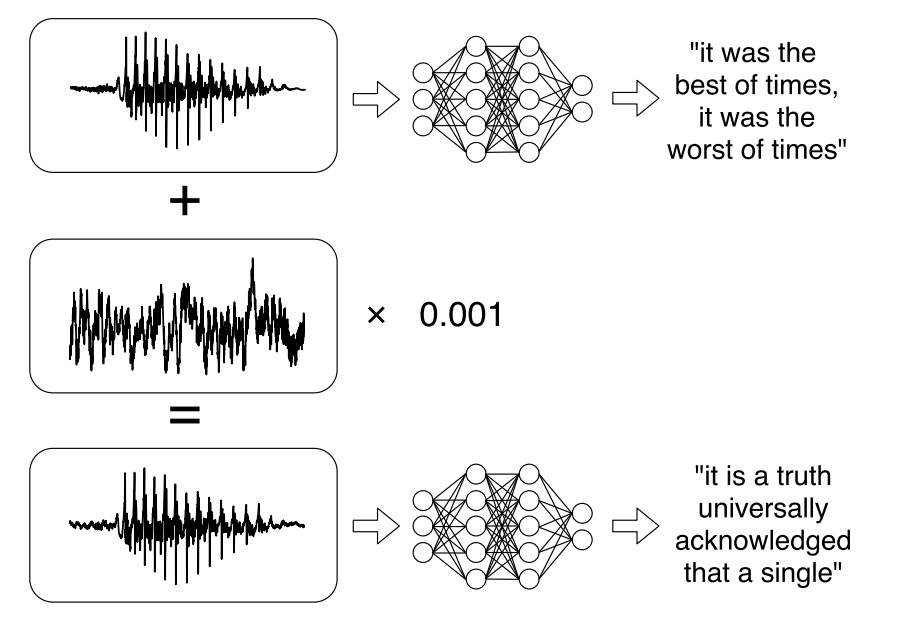
\includegraphics[height=4.5cm]{fig/yuying}
    \caption{语音错误识别}
    \label{fig:yuying}
\end{figure}

\subsubsection{超声波攻击}
利用麦克风在高频段的失真特性,攻击者将指令嵌入超声波\cite{roy2017inaudible}。人耳无法听到,但是麦克风会将其解析为有效语音命令,例如解锁手机、拨打电话等。此类攻击隐蔽性高,安全风险巨大。

\subsection{文本领域攻击案例}
\subsubsection{字符级对抗扰动}

在文本分类或情感分析任务中,只需替换若干字符或词语,就可误导模型输出\cite{ebrahimi2017hotflip, li2019textbugger}。例如“good”被替换为“g00d”或“goad”,看似仅是拼写错误,但是往往会使得模型判定成完全不同的情感标签。\autoref{tab:text_attack_example}给出了几个典型示例。

\begin{table}[htbp]
    \centering
    \caption{文本对抗样本}
    \label{tab:text_attack_example}
    \begin{tabular}{lll}
        \toprule
        原始文本 & 对抗样本 & 模型预测结果   \\
        \midrule
        This movie is fantastic! & This movie is fantastiic! & Negative \\
        I love this product.     & I luv th1s product.       & Negative \\
        \bottomrule
    \end{tabular}
\end{table}

在\autoref{tab:text_attack_example}中,微小的字符变化不会显著破坏句子可读性,人类读者仍可理解其原意,但情感分析模型可能将其错误地判定为负面评价\cite{li2019textbugger}。

\subsubsection{同义词替换与语义变换}
在文本对抗攻击中,同义词替换与语义变换是一种广泛应用且高效的攻击手段。其基本思想是针对文本中对模型决策具有较大影响的关键单词进行替换,使用具有相似语义但在模型内部表示略有不同的词汇,从而在不改变文本整体含义的前提下,干扰模型的特征捕捉。例如,\cite{li2019textbugger} 中展示了针对情感分析模型的攻击实验:原始文本 “This movie is fantastic!” 可能被替换为 “This movie is wonderful!” 或 “This movie is amazing!”。虽然这些词汇在日常语义中可以互换,但由于模型训练过程中不同词语的词向量存在细微差异,这种替换往往会导致预测结果发生显著偏差,从而使模型的分类结果从正面转为负面。

\section{攻击危害}
\zihao{5}\songti
\subsection{视觉领域的攻击危害}
在视觉领域,对抗样本对自动驾驶、监控安防和身份验证系统构成重大威胁。例如,自动驾驶系统依赖交通标志识别进行安全决策。通过对抗补丁攻击(Adversarial Patch),攻击者仅需在交通标志(如停车标志)上贴上特定干扰贴纸,便可能使系统将停车标志误判为限速标志,从而引发车辆误判、错误决策甚至交通事故\cite{brown2017adversarial, kurakin2018adversarial}。此外,面部识别系统也可能被对抗样本绕过,导致身份验证失效,进一步威胁公共安全\cite{sharif2016accessorize}。
\subsection{语音领域的攻击危害}
在语音领域,对抗攻击主要针对语音识别与语音助手系统。攻击者可通过在语音信号中注入微小但精心设计的扰动,生成隐蔽语音命令,使得设备在用户不知情的情况下执行错误操作。例如,Carlini 和 Wagner\cite{carlini2018audio}展示了如何通过音频对抗样本使语音识别系统输出错误文本,这可能导致智能音箱、车载语音系统等被远程控制、泄露隐私甚至触发未经授权的操作。由于这些扰动往往对人耳不可察觉,其实际危害更加难以防范。
\subsection{文本领域的攻击危害}
文本对抗攻击通过同义词替换、字符扰动和语义变换等手段,在保持文本整体语义一致的前提下,干扰文本分类、情感分析和自动审核系统。\cite{li2019textbugger}中实验表明,细微的词汇替换就能导致情感分析模型输出截然不同的结果。这种攻击不仅可能用于制造虚假信息,操纵舆情,还会影响金融风控、舆情监测等自动决策系统的稳定性和可信度。

\section{防御措施}
\zihao{5}\songti
\subsection{视觉领域的防御}
\subsubsection{对抗训练(Adversarial Training)}
在训练过程中将对抗样本加入训练集,使模型学会识别并抵抗扰动\cite{madry2018towards}。结合正则化与对抗训练,如TRADES\cite{zhang2019theoretically} 和 MART\cite{wang2020improving},在提高模型鲁棒性的同时尽量减少对精度的损害。
\subsubsection{输入变换与预处理}对输入图像进行随机裁剪、平移、噪声滤波、JPEG压缩等操作,使对抗扰动在预处理阶段被破坏\cite{xie2018mitigating, mustafa2019image}。该方案 实现简单,可与其他防御方法组合使用。但是某些自适应攻击可能针对预处理步骤进行绕过攻击。
\subsubsection{检测与过滤}
训练一个检测器识别输入是否包含对抗扰动\cite{metzen2017detecting}。若检测为对抗样本,则拒绝服务或进行额外处理。

\subsection{语音领域的防御}
\subsubsection{对抗训练与数据增强}
类似视觉领域的对抗训练,将音频对抗样本或加噪数据引入训练集中\cite{subramanian2019adversarial}。在保持模型准确率的同时,提升对高频扰动的鲁棒性。
\subsubsection{语音预处理与特征修正}
在语音输入阶段对信号进行降噪、量化、压缩或带通滤波等预处理\cite{yang2021analyzing}。 能有效削弱部分频域扰动,但是攻击者可针对该预处理过程设计自适应扰动,仍可能绕过。

\subsection{文本领域的防御}
\subsubsection{对抗训练与数据增强}
在训练集中加入多种文本扰动样本(如同义词替换、字符级噪声)\cite{jones2020robust}。该方式可以使模型学习到对微小字符或词汇变化的鲁棒性,但是需要不断更新数据增强策略以覆盖更多攻击方式。

\subsubsection{可解释模型与注意力修正}
在模型的注意力机制或特征提取层进行约束,使其对局部词汇变化不敏感\cite{wang2021infobert}。该方式通过限制注意力分布的突变来提升模型对字符或词汇替换的抵抗能力。

\subsubsection{对抗样本检测}
利用文本一致性检测或语言模型对流畅度与语义进行评估,识别异常字符和词汇的使用\cite{mozes2021freq}.

\section{个人对技术的理解}
\zihao{5}\songti
对抗样本攻击凸显了深度学习模型在高维空间中对微小扰动的极度敏感性,这是模型结构与训练机制所固有的脆弱性。通过对视觉、语音和文本三大领域的对抗案例进行研究,我进一步认识到以下几点:

防御技术(如对抗训练、随机平滑等)虽可减缓攻击影响,但自适应与迁移攻击的持续演进往往能绕过已有防御,反映出攻防博弈将长期存在。

不同场景对安全要求、实时性和资源限制各不相同,例如自动驾驶更注重物理可行性,语音系统需应对人耳听不出的高频扰动,文本系统则面临同义词替换等复杂语言现象。针对具体应用场景定制化的防御措施更具实用价值。





\bibliographystyle{IEEEtran}
\bibliography{Mybib}

\end{document}
